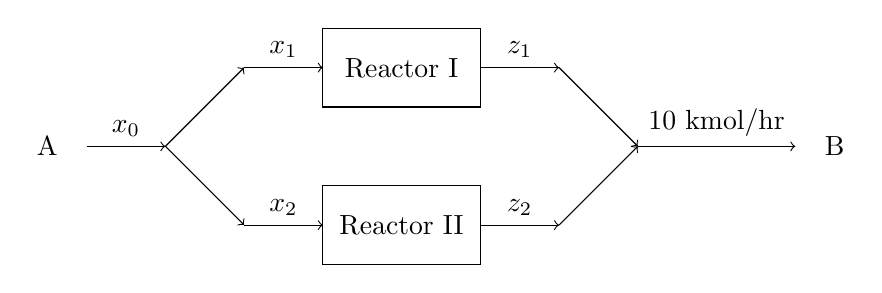
\begin{tikzpicture}
    % Reactor Boxes
    \draw (0,2) rectangle (2,3) node[pos=.5] {Reactor I};
    \draw (0,0) rectangle (2,1) node[pos=.5] {Reactor II};

    % Labels A and B
    \node at (-3.5, 1.5) {A};
    \node at (6.5, 1.5) {B};

    % Arrows and flows
    \draw[->] (-3, 1.5) -- (-2, 1.5) node[midway, above]{$x_0$} ;
    \draw[->] (-2,1.5) -- (-1,2.5);
    \draw[->] (-2,1.5) -- (-1,0.5);
    \draw[->] (-1,2.5) -- (0,2.5) node[midway, above] {$x_1$};
    \draw[->] (-1,0.5) -- (0,0.5) node[midway, above] {$x_2$};
    \draw[->] (2,2.5) -- (3,2.5) node[midway, above] {$z_1$};
    \draw[->] (2,0.5) -- (3,0.5) node[midway, above] {$z_2$};
    \draw[->] (3,2.5) -- (4,1.5);
    \draw[->] (3,0.5) -- (4,1.5);
    \draw[->] (4,1.5) -- (6,1.5) node[midway, above] {10 kmol/hr};

\end{tikzpicture}
